\chapter{Development prospects}

\section{Local modeling in a place}

Modeling inside places can be interesting to implement. However, it would not bring a major evolution in digitalization.\\

From a practical point of view, most epidemic simulations model balls bouncing off a rectangle. We can draw a parallel with a chaotic circulation of individuals in the same place. One could even add impassable shapes in the rectangle to represent the structural architecture in place. For example, one could design the parallel shelves of a supermarket. But again, it is very likely to fall into an overfitting of digitalization, which could weaken the robustness of epidemic modeling in scenarios.\\

In reality, the dynamic interest of such a consideration does not make it possible to provide more assurance on the relevance of contaminations in a place. Especially since no data could really support the momentum ; and it would probably be personal data, which would be unsympathetic in the eyes of individuals.\\

On the other hand, from a research point of view, it would be very interesting to study the ability of a place to promote proximity/contamination of its occupants depending on its architecture. In particular, in our digitalization project, it would be more than interesting to better define the contamination factors of the different categories of places.\\

\section{Exploring potential decisions}

Even if research places would explode, we could also increase combinatorial choices by replacing territorial decisions with the constraints of digitalization.\\

\section{Multi-territorial consideration}

We have to be caring. The consideration here will never be to be in a negative competition with the neighboring territory.\\

The idea is to optimize all territories in a global consideration. The major difference from the original modeling is the separation/duplication of the territory into several regions, each with independent decisions. The term "independent" is, however, to be looked at closely. We can find a form of game theory here, except that we do not want negative competition. From the point of view of benevolent optimization, only positive competition, where both develop, is to be considered. It should be noted that the consideration of interterritorial movements would have to be modified.\\

\section{Editing map data}

In a later version, it could be interesting to manually add places to extend the space for finding solutions to epidemic management. For example, there could be interest in building a new hospital, with a certain area and strategic location, to further optimize the management of infectious patients. We could then play on its location and area to observe its potential impact in digitalization. For this, we can use a Python package named \textit{Folium} that would position the correct strategic coordinates of the new place by observing the map of the area studied. Its category and area would remain to be defined. It would then be necessary to determine the nearest road, although it would be possible to discuss the connections between the location of the place and those of the roads in the network.\\

A very wide variety of possibilities can be found with this new consideration. The research space could explode if we add strategic decisions in static digitalization.\\

\section{Addition of the psychological criterion}

One of the avenues for evolution is also the addition of the psychological dimension to the management of the epidemic. We can see this with the reality of Covid-19 ; There is an increase in depression and suicide as a result of the major restrictions. Then, of course, we can question the real origin of psychological suffering. Do they come directly from territorial decisions ? In any case, it is obvious that the introduction of major restrictions such as lockdowns have impacted the psychological states of individuals. We could therefore try to find a form of psychological evaluation on the continuation of the decisions set. Indeed, there seems to be greater consistency in analyzing decisions in their succession rather than over a given time. We can also add the psychological factor of certain categories of places in the dynamics of individuals.\\

\section{In-depth analysis of results}

\begin{figure}[h]
  \centering
  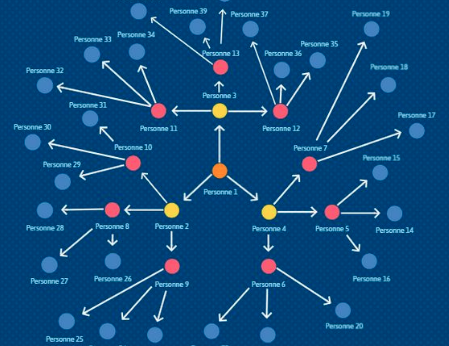
\includegraphics[width=0.8\linewidth]{media/r0.png}
  \caption{\centering {\small Epidemic propagation pattern.}}
  \label{fig:r0}
\end{figure}

In order to have more details on the design and to perfect the modeling, it may be more than interesting to determine epidemiological scores. For example, we could be interested in calculating the R0 scores of infections ; that is, the reproduction rate of the virus in society. This would give more guidance to better compare and parametrize infections in the implementation.\\

In general, it would be interesting to collect more data on epidemic digitalization to be able to tend digitalization towards observed infectious parameters. It would be a bit like gradient backpropagation in learning a neural network, more manually here.\\